% LTeX: enabled=false

\begin{titlepage} \centering

    % Logo y nombre de la facultad
    \begin{minipage}{0.6\textwidth}
        \begin{flushright}
            \LARGE \textbf{Universidad Nacional de Misiones} \par 
            \Large \textbf{Facultad de Ingeniería}
        \end{flushright}
    \end{minipage}
    \hspace{0.5 cm}
    \begin{minipage}{0.3\textwidth}
         
\includegraphics[width = 4 cm , height = 1.75 cm]{img/Logo_UNaM.png}
    \end{minipage}

    % Titulo
    \vspace{1 cm}
    \huge \textbf{Trabajo Práctico N.º 3}
    \par \vspace{-0.75 cm}
    \rule{\linewidth}{0.7 mm}

        \par \vspace{-0.5 cm}
        \Huge \textbf{KERALYTIX}

        \par \vspace{0.25 cm}
        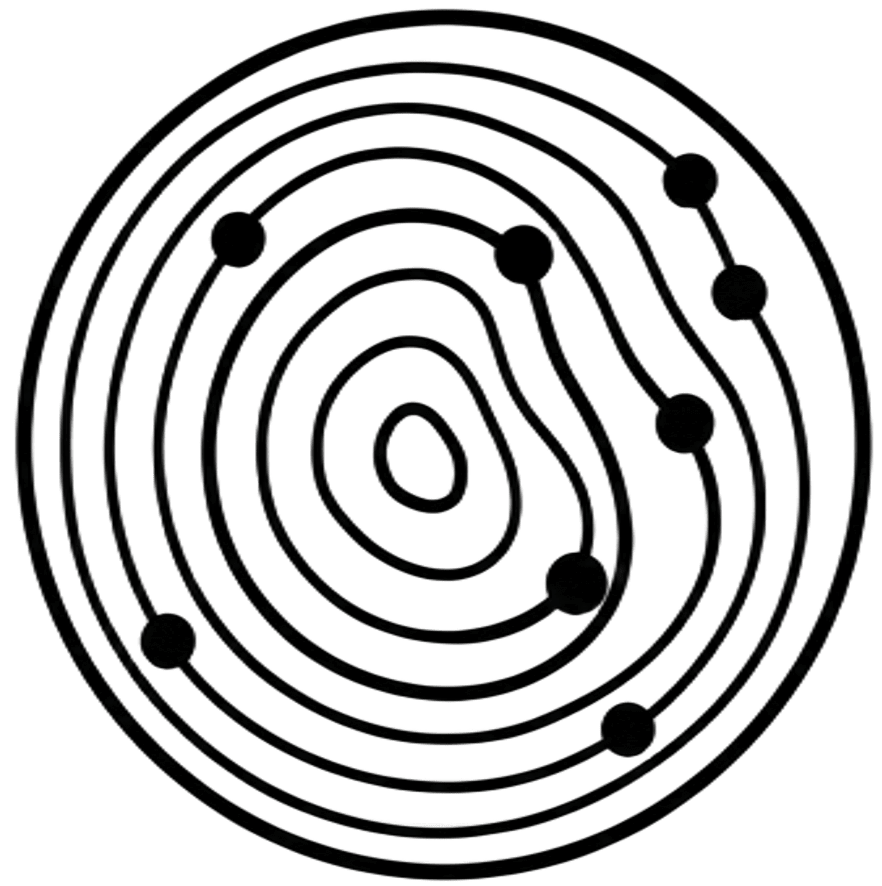
\includegraphics[width = 3 cm, height = 3 cm]{img/logotipo_solo.png}

        \large Sistema de soporte para la decisión clínica temprana del queratocono mediante IA multimodal

    \rule{\linewidth}{0.7 mm}

    % Grupo
    % \par \vspace{-1 cm}
    \textbf{\Large Grupo N.º 7}
    \vspace{0.2 cm}

    % Autores, Tutor y Docentes
    \begin{flushleft}
        \Large \textbf{Autores:} \par
        \Large \hspace{0.5 cm} Aranda, Brian Ezequiel \par
        \Large \hspace{0.5 cm} Wlodeck, Fabricio Joaquín  \par
        
        \vspace{0.25 cm}
        \Large \textbf{Docente tutor:} \par
        \Large \hspace{0.5 cm} Ing. Krujoski, Matías Gabriel\par
        
        \vspace{0.25 cm}
        \Large \textbf{Docentes de la cátedra:} \par
        \Large \hspace{0.5 cm} Dr. Ing. Javier Kolodziej \par
        \Large \hspace{0.5 cm} Dra. Ing. Romina Niezwida 
    \end{flushleft}
    \vspace{1.5 cm}

    % Fecha
    {\Large \textbf{Oberá, Misiones - 30 de octubre de 2026}} \par
    \Large \textbf{Cátedra: Proyecto final integrador [IC-522]} 
    
\end{titlepage}